
\begin{frame}
    \frametitle{Digitale signaalverwerking}

    \begin{figure}
        \centering
        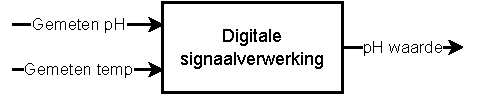
\includegraphics[width=\textwidth]{digitaalBlokje}
    \end{figure}

\end{frame}

\begin{frame}
    \frametitle{Digitale signaalverwerking}

    \begin{equation*}\label{eq:digitaleBS}
        pH = C_{pH}(\
            \only<2>{\colorbox{yellow}{$U_{pH}$}}\only<1,3->{U_{pH}}\
        - U_{pH,kal}) + C_T(\
            \only<3>{\colorbox{yellow}{$U_T$}}\only<-2,4->{U_T}\
        - U_{T,kal}) + pH_{kal}\
    \end{equation*}
    

    \pause[4]
    
    \begin{figure}
        \centering
        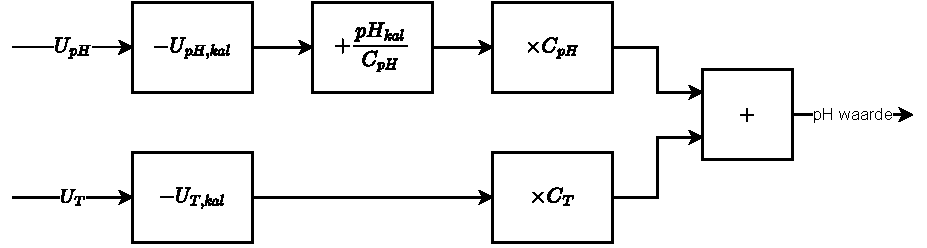
\includegraphics[width=\textwidth]{digitaleBewerkingsFunctie.pdf}
    \end{figure}
    % $\mathrm{CAL_{\mathrm{pH,H}}}=7$

    % $\mathrm{CAL_{\mathrm{pH,L}}}=4$

    % \begin{equation*}
    %     \mathrm{pH}=\frac{\mathrm{S}-\mathrm{CAL_{\mathrm{ADC,L}}}}{\mathrm{CAL_{\mathrm{ADC,H}}}-\mathrm{CAL_{\mathrm{ADC,L}}}}\left(\mathrm{CAL_{\mathrm{pH,H}}}-\mathrm{CAL_{\mathrm{pH,L}}}\right)+\mathrm{CAL_{\mathrm{pH,L}}}
    % \end{equation*}

\end{frame}